%% Sample dissertation using the kau_report LaTeX class
%%
%% 950203  Michael Kelsey -- LaTeX2e format (cit_thesis)
%% 990210  Anna Brunstrom -- Modified to KAU requirements
%% 990420  Anna Brunstrom -- Copyright page added + some minor updates

%\documentclass{kaumasters}
\documentclass[12pt,twoside]{Classfiles/kau_report}

\usepackage{float}
\PassOptionsToPackage{hyphens}{url}\usepackage{hyperref}
\usepackage{url}
\usepackage{subfig}
\usepackage{tabularx}
\usepackage{listings}
\usepackage{color}
\usepackage{pdfpages}
\usepackage{mathtools}
\usepackage{chngcntr}
\usepackage{pdfpages}
\usepackage[numbers]{natbib}
%\usepackage{refcheck}

\newcommand{\itab}[1]{\hspace{0em}\rlap{#1}}
\newcommand{\tab}[1]{\hspace{.2\textwidth}\rlap{#1}}
\newcommand\invisiblesection[1]{%
  \refstepcounter{section}%
  \addcontentsline{toc}{section}{\protect\numberline{\thesection}#1}%
  \sectionmark{#1}}

\AtBeginDocument{\counterwithin{lstlisting}{section}}

\setlength{\fboxsep}{0pt}

\definecolor{dkgreen}{rgb}{0, 0.6, 0}
\definecolor{gray}{rgb}{0.5, 0.5, 0.5}
\definecolor{mauve}{rgb}{0.58, 0, 0.82}
\lstset
{
	frame=tb,
	aboveskip=3mm,
	belowskip=3mm,
	showstringspaces=false,
	columns=flexible,
	basicstyle={\small\ttfamily},
	numbers=left,
	numberstyle=\color{gray},
	keywordstyle=\color{blue},
	commentstyle=\color{dkgreen},
	stringstyle=\color{mauve},
	breaklines=true,
	breakatwhitespace=true,
	tabsize=3,
}

% If you write in Swedish, uncomment line below
%\usepackage{swedish} %%Broken

% Define the parameters in the preamble

\title{Title of Dissertation\\ 
\large Subtitle of Dissertation of the most awesome theisis}
\swetitle{Examensarbetets Titel\\ 
\large Underrubrik till Examensarbetet av det hetaste Uppdraget}

\pubnum{June, 2016}
\swepubnum{Juni, 2016}

\author{Nicklas Hasselstr\"om}

\date{\today}

\advisor{Thijs. J. Holleboom}
\examiner{Donald F. Ross}

% The actual document starts here
\begin{document}
% Create the title page. If you write in swedish use the second line below instead.
\makekautitle
\makeswekautitle

%% Create the copyright page. If you write in swedish use the second line below instead.
\copyrightpage
%\swecopyrightpage

 %Start roman numbering
\begin{frontmatter}

% Create approval page. select the appropriate command depending
% on how many authors you have. If you write in swedish use 
% one of the sweapproved lines below instead.
%\approved
\approved
%\approvedthree{Author One}{Author Two}{Author Three}
%\sweapproved
%\sweapprovedtwo{Author One}{Author Two}
%\sweapprovedthree{Author One}{Author Two}{Author Three}

% Create abstract 
\begin{abstract}
%Motivation:

%Problem statement:

%Approach:

%Results:

%Conclusions:
English Abstract
\\
% KEYWORDS
\\
\textbf{Keywords:} My kewords


\end{abstract}
\cleardoublepage


% If you write in swedish you need a second abstract in  English. Uncomment lines below for the second absract.
\renewcommand{\abstractname}{Abstract (In Swedish)}
\begin{abstract}
%Motivation:
%Problem statement:
%Approach:
%Results:
%Conclusions:
Svensk Abstrakt
\\
% NYCEKLORD
\\
\textbf{Nyckelord:} Mina nyckelord

\end{abstract}
\cleardoublepage

% Create acknowledgements (optional part)
\begin{acknowledgements}
% If you want acknowledgements they go here
Tack alla
\end{acknowledgements}
\cleardoublepage

% Set up contents, list of figures and list of tables
  \tableofcontents
  \cleardoublepage

  \listoffigures
  \cleardoublepage

  \listoftables
  \cleardoublepage
  
  \lstlistoflistings
  \cleardoublepage

\end{frontmatter}
% End of roman numbering

% Here comes the main body, it's your job to fill this in...
\section{Introduction}
\label{sec:intro}
%Project goal and motivation
%Project summary & overview - the "red thread"
%Can you use a single Picture to give an overview of the project?
%Expected Results
%Project results (brief summary)
%Dissertation Layout


Intro Text
\cleardoublepage

\section{Background}
\label{sec:back}
%Introduce problem area / give relevant background info
%Introduction - Explain WHY you are doing this study
%Information - Background / your study in the wider context
%Similar work (projects, systems etc.)
%Chapter Summary
The human species is getting older and older. Our life span is getting longer which means that we have more time to get sick. The longer we live, the more likely it will be that we get one of the chronic diseases. In 2010 there were 759 million people over the age of 60. This was at the time 11 percent of the total population. In 2050 this group is estimated to be more than 2 billion. Not only does the population increase, proportionally the population is getting older and in 2050 it is estimated that 22 percent will be at the age of 60 and older~\cite{UNpub}.\\
With fewer people taking care of a growing population, new methods needs to be implemented in order to cover the lack of personnel. One of these new methods is home care. If a patient is well enough to care for them self, then it would take a huge burden of the welfare system. A patient who has been living with for example diabetes, knows how to do the daily check up, he knows how to take blood values and know best the state of his illness. If he can live a rich life at home and care for himself he will be happier and it will will free time which can be better spent on patients who need more care.\\
However, due to the age and progression of the disease of a patient, the health centre might want to keep a closer look at him and do daily check ups. Today this is done by sending a nurse to the home of a patient or by making the patient come to the health centre for daily and weekly check ups. This takes time from both the patient and nurse. If the the patient could send in data regarding their physical status this would greatly reduce the time of health care issues. One method which regards these problem is the Telehealth technology.\\

\subsection{Telehealth}
\label{sub:telehealth}
Telehealth~\cite{telehealth} is a collection of medical equipment used to monitor and collect data of the patient in his or her home. Data which is collected can be from blood pressure, blood values, weight, surveillance of demented patients or security alarm.\\
%Skriv mer här

\subsection{Tieto}
\label{sub:tieto}

\subsubsection{Lifecare eSense}
\label{subsub:eSense}

\subsubsection{Mobile gateway}
\label{subsub:gateway}

\subsection{Continua}
\label{sub:continua}

\subsection{Chapter Summary}
\label{sub:backSum}
\cleardoublepage

\section{Design}
\label{sec:design}
%Present your project design in general
%Can you use a single Picture to summarise your Design?
%Information - Give details here (possibly several sub-sections)
%Chapter Summary
Data flow
When the patient is doing an measurement with the medical equipment, data is generated in that device. This data is being sent to the mobile gateway over bluetooth and the gateway is acting like an server in this case, listening to transfer request from the medical device. If the medical device can not send its data, it stores it locally. The data is stored with all values and a timestamp of which time the measurement has been performed. 



Gateway - Medical Device interaction
Between the medical device and the phone the data is transmitted over bluetooth. The device must first pair with the phone and then the phone works as a server, waiting for data. This in line with the continua guideline on communication between continua certified units. To make this work, the Antidote framework was implemented.

Antidote
Antidote is an IEEE 11073 protocol stack library by signove. Signove is a company, working with connected health. They have implemented the library to provide simple communication between medical equipment. The library is open source and will work just fine in developing the prototype. To make the library work with teh application, it had to be build as a native library and then included in the project. Signove provided some sample applications for android, which were used in this project.

Antidote native build
The library is written in C so it has to be implemented with a bridge between the library and the application. Since the application is written in Java, the 

Gateway - eSense interaction

In Phone Functionality

Testing environment and data mocking

\cleardoublepage

\section{Implementation}
\label{sec:impl}
%Present your project implementation in general
%This should mirror the organisation of the Design chapter
%Information - Give details here (possibly several sub-sections)
%Chapter Summary

\subsection{Mobile gateway}
\label{sub:mobilegateway}
The main prototype of the thesis is an application which runs on an Android phone, it is the link between the medical device and the rest of the eSense. The application is written in Google Android which is essential the same as Java. The application have three different functionalities. Firstly it handles the connection to the medical device. This is done through Antidote, an open-source IEEE 11073-20601 stack. This stack is ported to android with the help of an JINI bridge and with the use of 

\cleardoublepage

\section{Results}
\label{sec:result}
%Introduction - Summarise your main results
%Give details of the results
%Best presentation? (text, tables, diagrams?)
%Implementation Evaluation - your results against your expectations
%Chapter Summary
Result text
\cleardoublepage

\section{Conclusions}
\label{sec:concl}
%o   Conclusion
%o   Project Evaluation
%o   Problems - How would you do this the next time?
%o   Future work
Concl text
\cleardoublepage

\nocite{*}

% Start of reference section. 
\begin{singlespace}
\bibliography{Appendices/myBibliography}
\bibliographystyle{apa}
\end{singlespace}
\cleardoublepage

% Appendix if present goes here (optional part)
\appendix
\section{Abbreviations}
\label{app:abbr}
\input{Appendices/abbreviations.tex}
\cleardoublepage

\section{Results}
\label{app:results}
Results goes here
\cleardoublepage

\section{Code}
\label{app:code}
See separate file.

%\subsection{Google Glass application}
%\label{app:code:ggApp}
%
%\lstinputlisting{ASW/BarcodeEye-master2/app/src/main/java/com/github/barcodeeye/AsyncResponse.java}
%\lstinputlisting{ASW/BarcodeEye-master2/app/src/main/java/com/github/barcodeeye/BaseGlassActivity.java}
%\lstinputlisting{ASW/BarcodeEye-master2/app/src/main/java/com/github/barcodeeye/Components.java}
%\lstinputlisting{ASW/BarcodeEye-master2/app/src/main/java/com/github/barcodeeye/DownloadProductTask.java}
%\lstinputlisting{ASW/BarcodeEye-master2/app/src/main/java/com/github/barcodeeye/GetService.java}
%\lstinputlisting{ASW/BarcodeEye-master2/app/src/main/java/com/github/barcodeeye/Instructions.java}
%\lstinputlisting{ASW/BarcodeEye-master2/app/src/main/java/com/github/barcodeeye/LaunchActivity.java}
%\lstinputlisting{ASW/BarcodeEye-master2/app/src/main/java/com/github/barcodeeye/Products.java}
%\lstinputlisting{ASW/BarcodeEye-master2/app/src/main/java/com/github/barcodeeye/ProductURL.java}
%\lstinputlisting{ASW/BarcodeEye-master2/app/src/main/java/com/github/barcodeeye/RandomizeEnglishText.java}
%\lstinputlisting{ASW/BarcodeEye-master2/app/src/main/java/com/github/barcodeeye/ServiceGenerator.java}
%\lstinputlisting{ASW/BarcodeEye-master2/app/src/main/java/com/github/barcodeeye/Timer.java}
%
%\lstinputlisting{ASW/BarcodeEye-master2/app/src/main/java/com/github/barcodeeye/image/ImageManager.java}
%
%\lstinputlisting{ASW/BarcodeEye-master2/app/src/main/java/com/github/barcodeeye/migrated/AmbientLightManager.java}
%\lstinputlisting{ASW/BarcodeEye-master2/app/src/main/java/com/github/barcodeeye/migrated/BeepManager.java}
%\lstinputlisting{ASW/BarcodeEye-master2/app/src/main/java/com/github/barcodeeye/migrated/DecodeFormatManager.java}
%\lstinputlisting{ASW/BarcodeEye-master2/app/src/main/java/com/github/barcodeeye/migrated/DecodeHintManager.java}
%\lstinputlisting{ASW/BarcodeEye-master2/app/src/main/java/com/github/barcodeeye/migrated/FinishListener.java}
%\lstinputlisting{ASW/BarcodeEye-master2/app/src/main/java/com/github/barcodeeye/migrated/HttpHelper.java}
%\lstinputlisting{ASW/BarcodeEye-master2/app/src/main/java/com/github/barcodeeye/migrated/InactivityTimer.java}
%\lstinputlisting{ASW/BarcodeEye-master2/app/src/main/java/com/github/barcodeeye/migrated/Intents.java}
%\lstinputlisting{ASW/BarcodeEye-master2/app/src/main/java/com/github/barcodeeye/migrated/LocaleManager.java}
%
%\lstinputlisting{ASW/BarcodeEye-master2/app/src/main/java/com/github/barcodeeye/scan/CaptureActivity.java}
%\lstinputlisting{ASW/BarcodeEye-master2/app/src/main/java/com/github/barcodeeye/scan/CaptureActivityHandler.java}
%\lstinputlisting{ASW/BarcodeEye-master2/app/src/main/java/com/github/barcodeeye/scan/CardScrollViewAdapter.java}
%\lstinputlisting{ASW/BarcodeEye-master2/app/src/main/java/com/github/barcodeeye/scan/DecodeHandler.java}
%\lstinputlisting{ASW/BarcodeEye-master2/app/src/main/java/com/github/barcodeeye/scan/DecodeThread.java}
%\lstinputlisting{ASW/BarcodeEye-master2/app/src/main/java/com/github/barcodeeye/scan/ResultsActivity.java}
%
%\lstinputlisting{ASW/BarcodeEye-master2/app/src/main/java/com/github/barcodeeye/scan/api/CardPresenter.java}
%\lstinputlisting{ASW/BarcodeEye-master2/app/src/main/java/com/github/barcodeeye/scan/api/DownloadImageTask.java}
%\lstinputlisting{ASW/BarcodeEye-master2/app/src/main/java/com/github/barcodeeye/scan/api/LoadImage.java}
%
%\lstinputlisting{ASW/BarcodeEye-master2/app/src/main/java/com/github/barcodeeye/scan/result/ResultProcessor.java}
%\lstinputlisting{ASW/BarcodeEye-master2/app/src/main/java/com/github/barcodeeye/scan/result/ResultProcessorFactory.java}
%
%\lstinputlisting{ASW/BarcodeEye-master2/app/src/main/java/com/github/barcodeeye/scan/result/internal/IsbnResultProcessor.java}
%\lstinputlisting{ASW/BarcodeEye-master2/app/src/main/java/com/github/barcodeeye/scan/result/internal/ProductResultProcessor.java}
%\lstinputlisting{ASW/BarcodeEye-master2/app/src/main/java/com/github/barcodeeye/scan/result/internal/TextResultProcessor.java}
%\lstinputlisting{ASW/BarcodeEye-master2/app/src/main/java/com/github/barcodeeye/scan/result/internal/UriResultProcessor.java}
%
%\lstinputlisting{ASW/BarcodeEye-master2/app/src/main/java/com/github/barcodeeye/scan/result/supplement/AmazonInfoRetriever.java}
%\lstinputlisting{ASW/BarcodeEye-master2/app/src/main/java/com/github/barcodeeye/scan/result/supplement/BookResultInfoRetriever.java}
%\lstinputlisting{ASW/BarcodeEye-master2/app/src/main/java/com/github/barcodeeye/scan/result/supplement/ProductResultInfoRetriever.java}
%\lstinputlisting{ASW/BarcodeEye-master2/app/src/main/java/com/github/barcodeeye/scan/result/supplement/SupplementalInfoRetriever.java}
%\lstinputlisting{ASW/BarcodeEye-master2/app/src/main/java/com/github/barcodeeye/scan/result/supplement/TitleRetriever.java}
%\lstinputlisting{ASW/BarcodeEye-master2/app/src/main/java/com/github/barcodeeye/scan/result/supplement/URIResultInfoRetriever.java}
%
%\lstinputlisting{ASW/BarcodeEye-master2/app/src/main/java/com/github/barcodeeye/scan/ui/ViewfinderView.java}
%
%\subsection{Smartphone application}
%\label{app:code:spApp}
%See separate file.
\cleardoublepage

\invisiblesection{Project Specification (In Swedish)}
\label{app:projectspec}
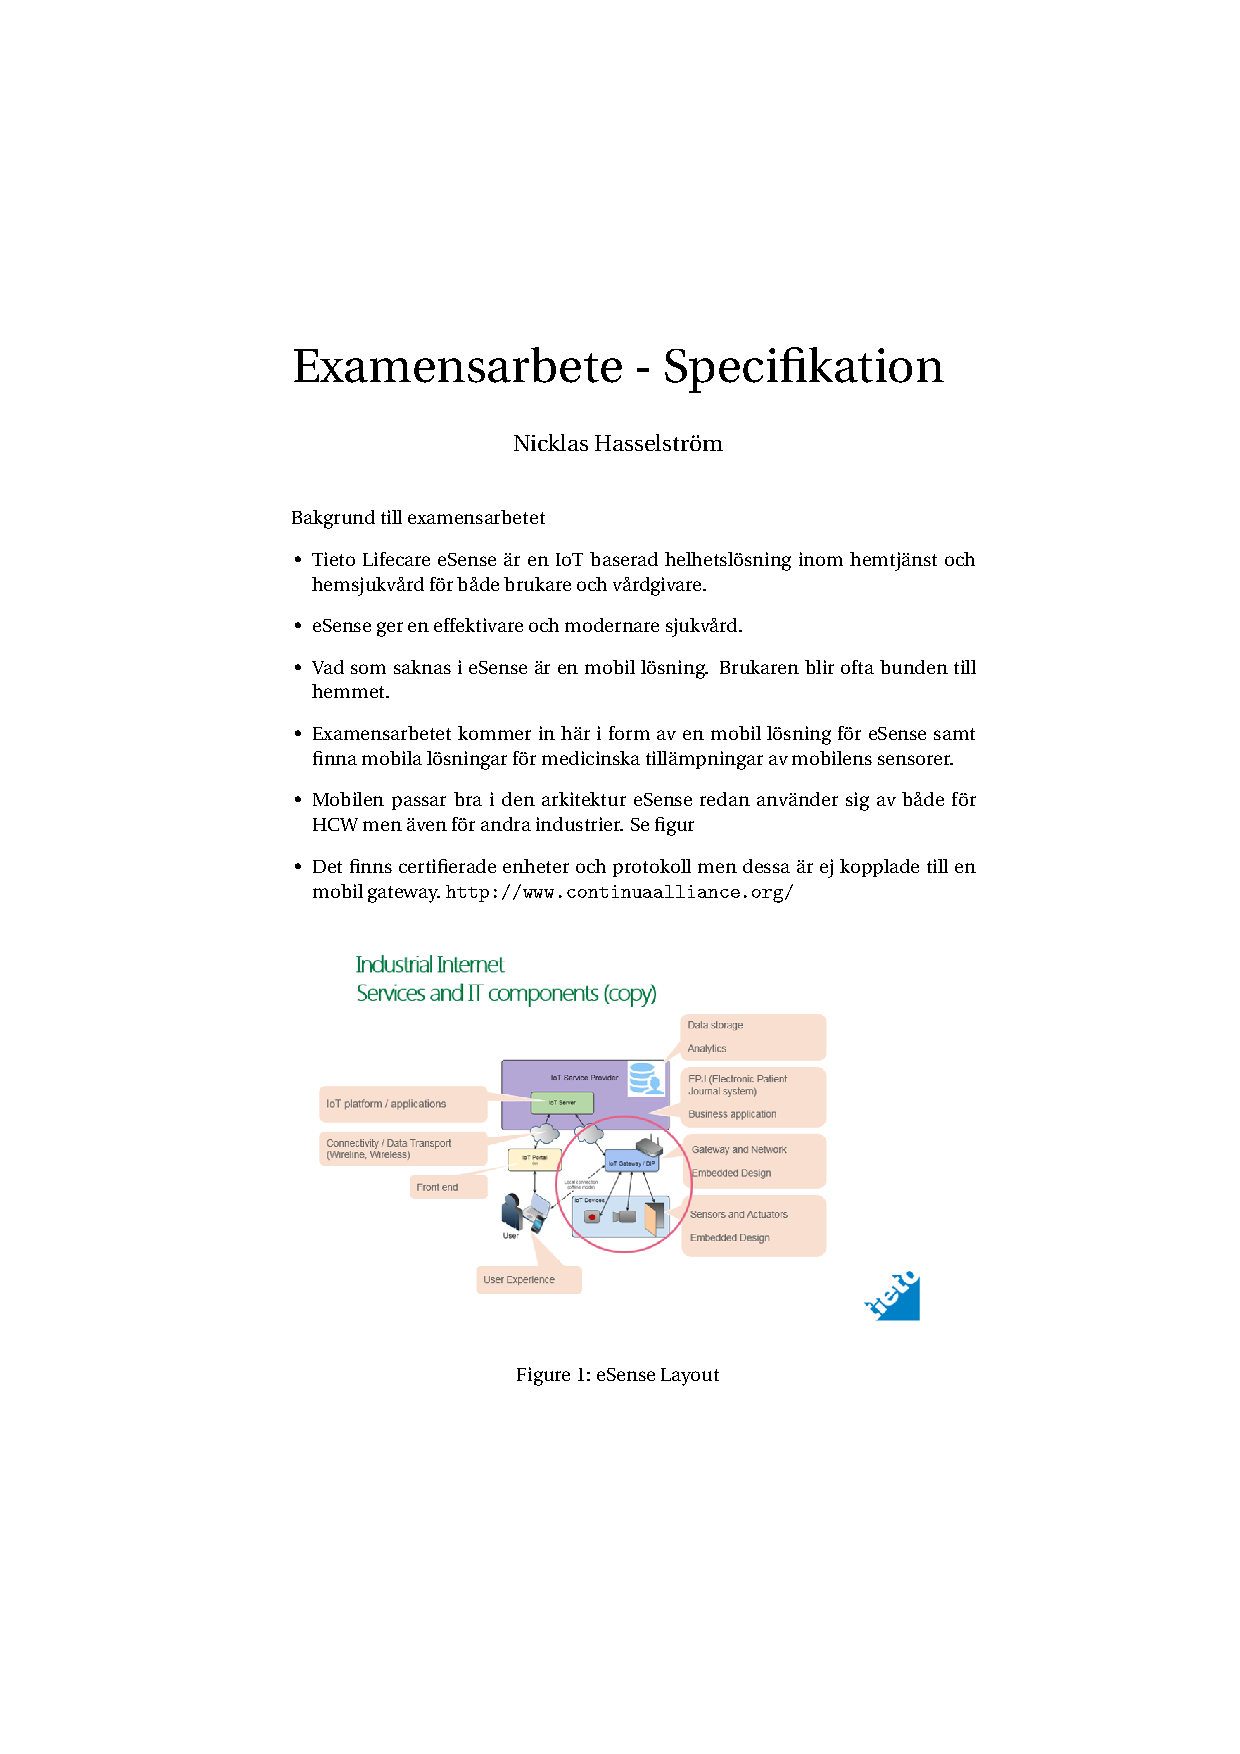
\includepdf[pages=-]{Appendices/Specifikation.pdf}

\end{document}
